\documentclass{article}
\usepackage{style}

\begin{document}

The cheatsheet will consist of the (1) defintions and theorems, (2) process, (3) canonical example with mark distribution. 

\section{Asymptotics}

\subsection{Big-O (Upper bound)}
\begin{definition}
    $ f(n) = O(g(n)) \text{ iff } \exists \text{ positive constants } c \text{ and } n_0 \text{ s.t. } 0 \leq f(n) \leq c g(n) \; \forall \; n \geq n_0 $
\end{definition}

\subsection{Big-Omega (Lower bound)}
\begin{definition}
    $ f(n) = \Omega(g(n)) \text{ iff } \exists \text{ positive constants } c \text{ and } n_0 \text{ such that } 0 \leq c g(n) \leq f(n) \; \forall \; n \geq n_0 $
\end{definition}

\subsection{Big-Theta (Tight bound)}
\begin{definition}
    \begin{enumerate}
        \item $ f(n) = \Theta(g(n)) \text{ iff } \exists \text{ positive constants } c_1, \; c_2, \; n_0 \text{ s.t. } 0 \leq c_1 g(n) \leq f(n) \leq c_2 g(n) \; \forall \; n \geq n_0 $
        \item $f(n) = \Theta(g(n))$ iff $f(n) = O(g(n))$ and $f(n)=\Omega(g(n))$.
    \end{enumerate}
\end{definition}

\subsection{Small-o (Strictly slower)}
\begin{definition}
    $f(n) = o(g(n)) \text{ iff } \forall c > 0, \exists n_0 > 0 \text{ s.t. } 0 \leq f(n) < c g(n) \text{ for all } n \geq n_0.$
\end{definition}

\subsection{Small-Omega (Strictly Faster)}
\begin{definition}
    $f(n) = \omega(g(n)) \text{ iff } \forall c > 0, \exists n_0 > 0 \text{ s.t. } 0 \leq c g(n) < f(n) \text{ for all } n \geq n_0.$
\end{definition}

\subsection{Comparing function properties}
\subsubsection{Transitivity:}
\begin{definition}
    \begin{itemize}
        \item $f(n) = \Theta(g(n)) \text{ and } g(n)=\Theta(h(n)) \text{ imply } f(n) = \Theta(h(n))$
        \item $f(n) = O(g(n)) \text{ and } g(n)=O(h(n)) \text{ imply } f(n) = O(h(n))$
        \item $f(n) = \Omega(g(n)) \text{ and } g(n)=\Omega(h(n)) \text{ imply } f(n) = \Omega(h(n))$
    \end{itemize}
\end{definition}

\subsubsection{Symmetry:}
\begin{definition}

    \textbf{Symmetry:}
    \begin{itemize}
        \item $f(n) = \Theta(g(n)) \text{ iff } g(n) = \Theta(f(n))$.
    \end{itemize}
    \vspace{1em}

    \textbf{Transpose symmetry:}
    \begin{itemize}
        \item $f(n) = O(g(n)) \text{ iff } g(n) = \Omega(f(n))$
    \end{itemize}
\end{definition}

\subsubsection{Common functions}
\begin{definition}
    \begin{enumerate}
        \item \( n^a = O(n^b) \), iff \( a \leq b \).
        \item \( \log_a(n) = O(\log_b(n)) \), $\forall$ \( a, b \).
        \item \( c^n = O(d^n) \), iff \( c \leq d \).
        \item If \( f(n) = O(f_1(n)) \) and \( g(n) = O(g_1(n)) \), then:
        \begin{enumerate}
            \item \( f(n) \cdot g(n) = O(f_1(n) \cdot g_1(n)) \).
            \item \( f(n) + g(n) = O(\max\{f_1(n), g_1(n)\}) \).
        \end{enumerate}
    \end{enumerate}
\end{definition}

\subsubsection{Comparing functions cookbook:}
\begin{definition}
    Assume 
    \begin{itemize}
        \item (1) \( f(n) \ll g(n) \) means \( f(n) = o(g(n)) \)
        \item (2) $f(n) \equiv g(n)$ means $f(n) = \Theta(g(n))$
        \item (3) \( f \) and \( h \) are eventually positive, i.e. \( \lim_{n \to \infty} f(n) > 0 \) and \( \lim_{n \to \infty} h(n) > 0 \). 
    \end{itemize}

    \begin{enumerate}
        \item \( 1 \ll \log^*(n) \ll \log^i n \ll (\lg n)^a \ll n^b \ll c^n \quad \forall i, a, b, c \)
        
        \item \( f(n) \ll g(n) \Rightarrow h(n)f(n) \ll h(n)g(n) \)
        
        \item \( f(n) \ll g(n) \Rightarrow f(n)^{h(n)} \ll g(n)^{h(n)} \)
        
        \item \( f(n) \ll g(n) \) and \( \lim_{n \to \infty} h(n) > 1 \Rightarrow h(n)^{f(n)} \ll h(n)^{g(n)} \)
    \end{enumerate}
\end{definition}

\subsection{Limit method}
\begin{definition}
    Find the asymptotic relationship between two functions for which you might not have any intuition about. 
    \begin{equation}
        \lim_{n \to \infty} \frac{f(n)}{g(n)} = 0 \Rightarrow f(n) = o(g(n))
    \end{equation}
    
    \begin{equation}
        \lim_{n \to \infty} \frac{f(n)}{g(n)} = \infty \Rightarrow f(n) = \omega(g(n))
    \end{equation}
    
    \begin{equation}
        \lim_{n \to \infty} \frac{f(n)}{g(n)} < \infty \text{ i.e. is anything finite } \Leftrightarrow f(n) = O(g(n))
    \end{equation}
    
    \begin{equation}
        \lim_{n \to \infty} \frac{f(n)}{g(n)} > 0 \text{ i.e. non-zero } \Leftrightarrow f(n) = \Omega(g(n))
    \end{equation}
    
    \begin{equation}
        \lim_{n \to \infty} \frac{f(n)}{g(n)} = C \text{ s.t. } 0 < C < \infty \Leftrightarrow f(n) = \Theta(g(n))
    \end{equation}        
\end{definition}

\subsection{Polynomially-bounded}
\begin{definition}
    \begin{itemize}
        \item \textbf{Polylogarithmically bounded:} \( f(n) = O((\lg n)^k) \quad \exists k > 0 \)
        
        \item \textbf{Polynomially bounded:} \( f(n) = O(n^k) \quad \exists k > 0 \)
        
        \item \textbf{Exponentially bounded:} \( f(n) = O(k^n) \quad \exists k > 0 \)
    \end{itemize}
\end{definition}

\begin{theorem}
    $f(n) = O(n^k) \Leftrightarrow \lg(f(n)) = O(\lg n)$
\end{theorem}

\begin{theorem}
    All logarithmically bounded functions are polynomially bounded, i.e. \((\lg n)^a = O(n^b) \quad \forall a, b > 0\)
\end{theorem}

\begin{theorem}
    All polynomially bounded functions are exponentially bounded, i.e. \( f(n) = O(n^a) \Rightarrow f(n) = O(b^n) \quad \forall a > 0 \text{ and } \forall b > 1\)
\end{theorem}

\subsection{Logarithm method}
\subsubsection{Limits of logs are logs of limits}
\begin{definition}
    $\lim_{x \to a} (\log_b f(x)) = \log_b \left( \lim_{x \to a} f(x) \right)$
\end{definition}

\begin{process}
    $\text{Suppose we want to compute } \lim_{n \to \infty} \frac{f(n)}{g(n)} = L$
    \begin{enumerate}
        \item \textbf{Take log of limit:}
        \begin{equation*}
            \lg \left( \lim_{n \to \infty} \frac{f(n)}{g(n)} \right) = \lg L
        \end{equation*}
        \item \textbf{Change to limit of log and compute it:}
        \begin{equation*}
            \lim_{n \to \infty} \left( \lg \frac{f(n)}{g(n)} \right) = \lg L 
        \end{equation*}
        \item \textbf{Revert log by taking exponential with base 2:}
        \begin{equation*}
            \lim_{n \to \infty} \frac{f(n)}{g(n)} = 2^{\lg L} = L
        \end{equation*}
    \end{enumerate}
\end{process}

\newpage

\section{Logarithms}
\begin{definition}
    \begin{equation}
        a = b^c \iff \log_b a = c
    \end{equation}
    \begin{itemize}
        \item Always assume base 2.
    \end{itemize}
\end{definition}

\subsection{Properties}
\begin{definition}
    $\forall \text{ real } a>0 \text{, } b>0 \text{, } c>0, \text{ and } n, \text{ we have}$
    \begin{enumerate}
        \item \( a = b^{\log_b a} \)
        \item \( \log_c(ab) = \log_c a + \log_c b \)
        \item \( \log_b a^n = n \log_b a \)
        \item \( \log_b a = \frac{\log_c a}{\log_c b} \)
        \item \( \log_b \left(\frac{1}{a}\right) = -\log_b a \)
        \item \( \log_b a = \frac{1}{\log_a b} \)
        \item \( a^{\log_b c} = c^{\log_b a} \)
        \item \( \log_b \frac{a}{c} = \log_b a - \log_b c\)
    \end{enumerate}
\end{definition}

\subsection{Logarithm iteration}
\begin{definition}
    $\log(n)$ iteratively applied $i$ times to an initial value of $n$.
    \begin{equation}
        \log^{(i)}(n) = 
        \begin{cases}
            n & \text{iff } i = 0, \\
            \log\left(\log^{(i-1)}(n)\right) & \text{if } i > 0.
        \end{cases}
    \end{equation}
\end{definition}

\subsection{Iterated logarithm function}
\begin{definition}
    The minimum number of times \( i \) that the logarithm function must be applied to \( n \) for the result to be less than or equal to 1:
    \begin{equation}
        \lg^{*} n = \min \left\{ i \geq 0 \; : \; \lg^{(i)} n \leq 1 \right\}
    \end{equation}
\end{definition}

\begin{warning}
    $O(n\log^* n) \approx O(n)$
\end{warning}

\newpage

\section{Summations}
    \subsection{Fibonacci Numbers}
        \begin{definition}
            \begin{equation}
                F_i = 
                \begin{cases}
                    0 & \text{if } i = 0, \\
                    1 & \text{if } i = 1, \\
                    F_{i-1} + F_{i-2} & \text{if } i \geq 2.
                \end{cases}
            \end{equation}
        \end{definition}

    \subsection{Arithmetic series}
        \begin{definition}
            \begin{equation}
                \sum_{k=1}^{n} k = \frac{n(n+1)}{2} = \Theta(n^2)
            \end{equation}
        \end{definition}

    \subsection{General arithmetic series}
        \begin{definition}
            For $a \geq 0 \text{ and } b > 0$,
            \begin{equation}
                \sum_{k=1}^{n} (a + bk) = \Theta(n^2)    
            \end{equation}
        \end{definition}

    \subsection{Sum of squares}
        \begin{definition}
            \begin{equation}
                \sum_{k=0}^{n} k^2 = \frac{n(n+1)(2n+1)}{6}
            \end{equation}
        \end{definition}

    \subsection{Sum of cubes}
        \begin{definition}
            \begin{equation}
                \sum_{k=0}^{n} k^3 = \frac{n^2(n+1)^2}{4}
            \end{equation}
        \end{definition}

    \subsection{Finite geometric series}
        \begin{definition}
            For $x \neq 1$, 
            \begin{equation}
                \sum_{k=0}^{n} x^k = 1 + x + \ldots + x^n  = \frac{x^{n+1} - 1}{x-1} 
            \end{equation}
        \end{definition}

    \subsection{Infinite decreasing geometric series}
        \begin{definition}
            For $\abs{x} < 1$, 
            \begin{equation}
                \sum_{k=0}^{\infty} x^k = \frac{1}{1-x}
            \end{equation}
        \end{definition}

    \subsection{Harmonic series}
        \begin{definition}
            For positive integers $n$, the $nth$ harmonic number is
            \begin{equation}
                \sum_{k=1}^{n} \frac{1}{k} = \ln n + O(1)
            \end{equation}                
        \end{definition}

    \subsection{Telescoping series}
        \begin{definition}
            For any sequence $a_0, a_1, \text{ ... }, a_n$,

            \begin{equation}
                \sum_{k=1}^{n} (a_k - a_{k-1}) = a_n - a_0 \quad \text{ OR } \quad \sum_{k=0}^{n-1} (a_k - a_{k+1}) = a_0 - a_n
            \end{equation}
        \end{definition}

    \subsection{Reindexing summations}
        \begin{process}
            \begin{enumerate}
                \item \textbf{Start with the original sum}
                \[
                S = \sum_{k=a}^{b} f(k)
                \]

                \item \textbf{Introduce a new variable:} Let the new variable $\ell$ be defined in terms of the old variable $k$, $\ell = g(k)$

                \item \textbf{Substitute the new variable into the sum:} $f(k) = h(\ell)$

                \item \textbf{Adjust the limits of summation:} When $k = a$, $\ell = g(a)$, and when $k = b$, $\ell = g(b)$.

                \item \textbf{Rewrite the summation in terms of the new variable:}
                \[
                S = \sum_{\ell = g(a)}^{g(b)} h(\ell)
                \]
            \end{enumerate}

            \begin{itemize}
                \item \textbf{Intuition:} If the summation index appears in the body of the sum with a minus sign, it's worth thinking about reindexing.
            \end{itemize}
        \end{process}
\newpage

\section{Induction, Contradiction, \& Combinatorial Arguments}
\subsection{Direct proof}
\begin{process}
    \begin{enumerate}
        \item Start with the givens
        \item Mathematically manipulate the givens and/or reason about the givens to arrive at the conclusion.
    \end{enumerate}
\end{process}

\subsection{Weak Induction}
\begin{process}
    Given predicate $P(n)$
    \begin{enumerate}
        \item \textbf{Basis Step:} Prove $P(n_0)$ for some value $n_0$. 
        \item \textbf{Hypothesis:} Assume $P(k)$ is true for $n=k$.
        \item \textbf{Inductive step:} Use the hypothesis $P(k)$ to show its true for $n=k+1$ s.t. $P(k+1)$.
    \end{enumerate}
    Therefore, $\forall n \geq n_0 \text{, } P(n)$ is true.
\end{process}

\subsection{Strong Induction}
\begin{process} 
    Given predicate $P(n)$
    \begin{enumerate}
        \item \textbf{Basis:} Show \( P(n_0), P(n_1), \ldots \) are true.
        \item \textbf{Hypothesis:} Assume \( P(k) \) is true, \( \forall k \leq n \).
        \item \textbf{Step:} Use the hypothesis \( P(n_0) \land \cdots \land P(k) \land \cdots \land P(n)\) to show its true for \( P(k+1) \).
    \end{enumerate}    
\end{process}

\subsection{Contradiction}
\begin{process}
    Given predicate $P(n)$ either true or false.
    \begin{enumerate}
        \item Assume toward a contradiction $\neg P(n)$.
        \item Make some argument by working with the expression $\neg P(n)$ to get to a contradiction.
        \item Arrive at a contradiction
        \item If this resulted in a contradiction then $P(n)$ is true. 
    \end{enumerate}
\end{process}

\subsection{Combinatorial argument}
\begin{process}
    \begin{enumerate}
        \item \textbf{Question:} Ask a question relating to the formula you would like to prove. Choose the easier side to start and make the question based on this side.
        \item \textbf{LHS:} Argue why the LHS answers the question.
        \item \textbf{RHS:} Argue why the RHS answers the question.
    \end{enumerate}
\end{process}

\begin{intuition}
    \begin{itemize}
        \item $+$: Or event
        \item $\cdot$: And event
        \item Subtracting inside a combination usually means were \textbf{excluding} or \textbf{removing} objects.
    \end{itemize}
\end{intuition}
\newpage

\section{Recurrences and the Master Theorem}
\subsection{Master Theorem}
\begin{theorem}
    Let \( a \geq 1 \), \( b > 1 \), and \( f(n) \) be a function, so that the recurrence is 

    \begin{equation}
        T(n) = aT\left(\frac{n}{b}\right) + f(n)
    \end{equation}

    Then the asymptotic behavior of \( T(n) \) is
    \begin{enumerate}
        \item If \( f(n) = O\left(n^{\log_b (a) - \epsilon}\right) \) for \( \epsilon > 0 \), then \( T(n) = \Theta\left(n^{\log_b a}\right) \).
        
        \item If \( f(n) = \Theta\left(n^{\log_b (a)}\right) \), then \( T(n) = \Theta\left(n^{\log_b a} \log n\right) \).
        
        \item If \( f(n) = \Omega\left(n^{\log_b (a) + \epsilon}\right) \) for \( \epsilon > 0 \) and \( af\left(\frac{n}{b}\right) \leq cf(n) \) for \( 0 < c < 1 \), then \( T(n) = \Theta(f(n)) \).
    \end{enumerate}
\end{theorem}

\begin{process}
    \begin{enumerate}
        \item Identify $T(n)$
        \item State $a$, $b$, and $f(n)$. Make sure the conditions are met.
        \item Calculate $n^{\log_b a}$. 
        \item Compare $f(n)$ with $n^{\log_b a}$ to see which case the function applies too.
        \begin{enumerate}
            \item If $\epsilon$ case is used, then apply an abitrary value to see (usually natural numbers work well).
        \end{enumerate}
        \item Write down the answer with the corresponding case.
    \end{enumerate}
\end{process}

\subsection{Substitution}
\begin{process}
    \begin{enumerate}
        \item Guess the form of the solution for $T(n)=?$ (given on a test)
        \item Use induction to show that the solution works.
        \begin{enumerate}
            \item Basis: Find the base case using values of n that correspond (i.e. make sense) with the guessed solution.
            \item Inductive hypothesis:
            \item Inductive step:
        \end{enumerate}
        \item Find the constants.
    \end{enumerate}
\end{process}

\subsection{Recursion tree}
\begin{process}
    \begin{enumerate}
        \item Draw a recursion tree using $T(n)$ and split it off into the other $T$'s.
        \item Sum the work within each level of the tree to obtain the per-level work.
        \item Determine the height, which is $r^h n = 1$ 
        \begin{itemize}
            \item 1: When the recursion problem size is 1. 
            \item $r$: Largest value child from the root. 
            \item $n$: Initial problem size
            \item \textbf{Key:} The root's children bigger value determines the height of the tree as it will reach $O(1)$ (i.e. base-case) the slowest compared to the other branch, making it the longest path in the recursion tree. 
        \end{itemize}
        \item Determine the total work: $h \cdot \text{Work done at every level}$ 
    \end{enumerate}
\end{process}
\newpage

\section{Graphs}
\begin{definition}
    $G = (V, E)$, where $V = \{\text{vertices}\}$ and $E = \{\text{edges}\}$.
\end{definition}

\subsection{Directed and Undirected, Weighted Graphs}
\begin{terminology}
    \begin{itemize}
        \item \textbf{Directed graph (digraph):} Each edge has a direction from one vertex to another. 
        \begin{itemize}
            \item \textbf{Edges:} $(v_1,v_2)$ and $(v_2,v_1)$ are different.
            \item \textbf{Self-loop:} Edges from a vertex to itself.
            \item \textbf{In/Out Degree of V:} Out-degree is the \# of edges leaving it, while in-degree is the \# of edges entering it.
            \item \textbf{Degree of V:} In-degree plus out-degree.
        \end{itemize}
        \item \textbf{Undirected graph:} Each edge does not have a specific direction.
        \begin{itemize}
            \item \textbf{Edges:} $(v_1,v_2)$ and $(v_2,v_1)$ are indifferent.
            \item \textbf{Self-loop:} Forbidden.
            \item \textbf{Degree of V:} Number of edges incident on it.
        \end{itemize}
        \item \textbf{Weighted graph:} A graph where each edge is associated with a value (e.g. distance, profit, penalty).
        \item \textbf{Simple graph:} Graph with no self-loops, or multi-edges.
        \item \textbf{Induced graph:} Subset of $G$ and the associated edges.
        \item \textbf{Spanning subgraph:} Let $G' = (V',E')$ be a subgraph of $G=(V,E)$, $G'$ is a spanning subgraph if $V'=V$.
    \end{itemize}
\end{terminology}
        
\subsection{Paths and cycles}
    \begin{terminology}
        \begin{itemize}
            \item \textbf{Path:} Going from one vertex to another. 
            
            \item \textbf{Simple Path:} A path with no repetition of vertices.
            
            \item \textbf{Cycle:} A path that begins and ends at the same vertex, which can pass through the same vertex multiple times.

            \item \textbf{Simple Cycle:} A path that begins and ends at the same vertex, with no other repeated vertices.
        \end{itemize}
    \end{terminology}
    
\subsection{AG, DAG}
    \begin{terminology}
        \begin{itemize}
            \item \textbf{Acyclic Graph:} A graph with no cycles is an acyclic graph.
            \item \textbf{Directed Acyclic Graph:} A DAG is a directed acyclic graph. 
        \end{itemize}
    \end{terminology}

\subsection{Connected, disconnected graph}
    \begin{terminology}
        \begin{itemize}
            \item \textbf{Connected:} Two vertices are connected if there is a path between them.
            \item \textbf{Connected graph:} $\exists$ path between $\forall \; 2$ vertices.
            \item \textbf{Disconnected graph:} $\exists$ at least one pair of vertices such that no path exists between them.
        \end{itemize}
    \end{terminology}

\subsection{Bipartite Gs}
    \begin{definition}
        $V$ can be partitioned into $2$ sets $V_1$ and $V_2$ s.t. $V_1 \cap V_2 = \emptyset$ and $V_1 \cup V_2 = V$ and adjacencies only between elements of $V_1$ and $V_2$.
    \end{definition}

\subsection{Clique (complete G)}
\begin{definition}
    $\exists$ edge between $\forall \; 2$ vertices. 
    \begin{equation}
        \# edges = \frac{V(V-1)}{2} = \binom{V}{2}
    \end{equation}
\end{definition}

\subsection{Degrees of all V}
\begin{definition}
    \begin{equation}
        \sum_{v\in V} degree(v) = 2\abs{E}
    \end{equation}
\end{definition}

\subsection{Graph representation}
\begin{definition}
    
    \textbf{Adjacency matrix (AM):} An $n\times n$ matrix where $M[i][j]=1$ if there is an edge between $v_i$ and $v_j$, and $0$ otherwise (undirected) or $M[i][j]=1$ if there is an edge from $v_i$ to $v_j$, and $0$ otherwise (directed).
    \begin{itemize}
        \item \textbf{Time to search for E:} $O(1)$ (i.e. since in matrix format)
        \item \textbf{Memory space:} $O(V^2)$ (i.e. matrix has $x^2$ entries)
        \item Good for dense $G$ (i.e. $E>>V^2$)
        \item For a directed graph, when you take the transpose of $G$, you get the complement of the original graph.
    \end{itemize}
    \vspace{1em}

    \textbf{Adjacency list (AL):} For $n=\abs{V}$ vertices, $n$ linked lists. The $ith$ linked list, $L[i]$ is a list of all the vertices that are adjacent to vertex $i$.
    \begin{itemize}
        \item \textbf{Time to search for E:} $O(V)$ (i.e. may be on the last vertex)
        \item \textbf{Memory space:} $O(V+E)$ (i.e. store all the vertices and edges once)
        \item Good for sparse $G$ (i.e. $E<<V^2$).
    \end{itemize}
    \vspace{1em}
\end{definition}
\newpage

\section{Trees}
\begin{definition}
    A tree is a connected, acyclic, undirected graph. 
\end{definition}

\subsection{Properties}
\begin{definition}
    Let $G=(V,E)$ be an undirected graph. The following statements are equivalent:
    \begin{enumerate}
        \item $G$ is a tree. 
        \item Any two vertices in $G$ are connected by a unique simple path. 
        \item $G$ is connected, but if any edge is removed from $E$, the resulting graph is disconnected. 
        \item $G$ is connected, and $\abs{E} = \abs{V} - 1$.
        \item $G$ is acyclic, and $\abs{E} = \abs{V} - 1$.
        \item $G$ is acyclic, but if any edge is added to $E$, the resulting graph contains a cycle.
    \end{enumerate}
\end{definition}

\subsection{Terminology}
\begin{terminology}
    \begin{itemize}            
        \item \textbf{Parent:} A node \( y \) is the parent of node \( x \) if \( y \) is directly connected to \( x \) on the path from the root.
        
        \item \textbf{Child:} A node \( x \) is a child of node \( y \) if \( y \) is the parent of \( x \).
        
        \item \textbf{Siblings:} Nodes are siblings if they share the same parent.
        
        \item \textbf{Leaf (or External Node):} A leaf is a node with no children.
        
        \item \textbf{Internal Node:} An internal node is a nonleaf node, which means it has at least one child.
        
        \item \textbf{Degree:} The degree of a node \( x \) is the number of children it has.
        
        \item \textbf{Level:} A level of a tree consists of all nodes at the same depth.
        
    \end{itemize}
\end{terminology}

\subsection{Height, depth}
\begin{definition}
    \begin{itemize}
        \item \textbf{Depth:} The depth of a node \( x \) is the number of edges from the root to \( x \).
        
        \item \textbf{Height:} The height of a node is the number of edges in the longest path from that node to a leaf.
        \begin{itemize}
            \item \textbf{Height of tree:} From root to any leaf.
        \end{itemize}
    \end{itemize}

\end{definition}

\subsection{K-ary trees}
\begin{definition}
        Each $\text{node} \leq k$ children. A binary tree has \( k = 2 \).
        \vspace{1em}

        A \textbf{complete k-ary tree} is a k-ary tree in which all leaves have the same depth, and every internal node has exactly \( k \) children. 
\end{definition}
\newpage

\section{Permutations, Combinations}
\subsection{Rule of sum and product}
    \begin{definition}
        If there are m-ways for event $A$ to happen and n-ways for event $B$ to happen then\dots
        \vspace{1em}

        \textbf{Rule of product:} $\exists \; m\times n$ ways for $A$ \emph{and} $B$ to happen. 
        \vspace{1em}

        \textbf{Rule of sum:} $\exists \; m + n$ ways for $A$ \emph{or} $B$ to happen. 
    \end{definition}

\subsection{Factorials}
    \begin{definition}
        Number of ways to arrange $n$ distinct objects when order is important.
        \begin{equation}
            n! = n(n-1)(n-2)\cdots 2\cdot 1
        \end{equation}
    \end{definition}
    
\subsection{Permutations}
    \begin{definition}
        Number of ways to pick $r$ distinct objects out of $n$ where \emph{order matters} and \emph{repetition isn't allowed}.
        \begin{equation}
            P(n,r) = n(n-1)(n-2)\cdots(n-r+1) = \frac{n!}{(n-r)!} 
        \end{equation}
        \begin{itemize}
            \item $n$: total number of elements in the set.
            \item $r$: number of elements taken from the set.
        \end{itemize}
    \end{definition}

\subsection{Permutations with identical items}
    \begin{definition}
        If there are $m$ kinds of items and $q_k$, $k=1,\ldots,m$ of each kind, then total number of permutations where \emph{order matters} is 
        \begin{equation}
            \binom{n}{q_1, \ldots, q_m} = \frac{n!}{q_1! \, q_2! \, \cdots \, q_m!}
        \end{equation}
        \begin{itemize}
            \item $\sum_{k=1}^{m} q_k = n$
        \end{itemize}
    \end{definition}

\subsection{Permutations with repetitions}
    \begin{definition}
        Number of ways to arrange \( r \)-objects out of \( n \) objects with unlimited repetition is given by: $n^r$.
    \end{definition}

\subsection{Combinations}
    \begin{definition}
        Number of ways to choose $r$ objects from $n$ where \emph{order doesn't matter}. 
        \begin{equation}
            C(n,r) = \binom{n}{r} = \frac{P(n,r)}{r!} = \frac{n!}{r!(n-r)!}
        \end{equation}
    \end{definition}

\newpage

\section{Probability}
\subsection{Sample space}
    \begin{definition}
        The set of \emph{all possible outcomes} of a statistical experiment, denoted by $S$.
    \end{definition}

\subsection{Event}
    \begin{definition}
        A subset of a sample space $S$. An event is any outcome or combination of outcomes.
    \end{definition}

\subsection{Probability axioms}
    \begin{definition}
        For $A$, $B \subseteq S$
        \begin{enumerate}
            \item $0 \leq P(A) \leq 1$
            \item $P(S) = 1$
            \item $P(A \cup B) = P(A) + P(B)$ for two mutually exclusive events $A$ and $B$. 
        \end{enumerate}
    \end{definition}

\subsection{Mutually exclusive events}
\begin{definition}
    $\text{If } A_1, A_2, A_3, \dots \text{ is a sequence of mutually exclusive events, then}$
    \begin{equation}
        P(A_1 \cup A_2 \cup A_3 \cup \dots) = P(A_1) + P(A_2) + P(A_3) + \dots    
    \end{equation}
    \begin{itemize}
        \item \textbf{Key}: Independent is \textbf{NOT} mutually exclusive.
        \item \textbf{Key Implication}: For independent events, we can multiply their probabilities to get their intersection (useful for \textbf{calculating favorable outcomes}).
        \begin{itemize}
            \item \( P(A \cap B \cap C \cap D) = P(A)P(B)P(C)P(D) \) \text{ as long as they are \textbf{INDEPENDENT}.}
            \item \textbf{Note}: Can also be applied to a sequence of dependent events as long as you adjust for changing conditions.
        \end{itemize}
    \end{itemize}
\end{definition}

\subsection{Additive rule}
    \begin{definition}
        \begin{equation}
            P(A \cup B) = P(A) + P(B) - P(A\cap B)
        \end{equation}
    \end{definition}

\subsection{Uniform distribution}
    \begin{definition}
        If $\forall s\in S$ has probability $P(s) = \frac{1}{\abs{S}}$, then it is a uniform distribution.
    \end{definition}

\subsection{Independence}
    \begin{definition}
        $P(A \cap B) = P(A)P(B)$ if $A$, $B$ independent.
    \end{definition}

\subsection{Bayes theorem}
    \begin{definition}
        For events with $P(A)>0$ and $P(B)>0$, the probability $A$ happens given $B$ happens is:
        \begin{equation}
            P(B|A) = \frac{P(B\cap A)}{P(A)} = \frac{P(A|B)P(B)}{P(A)}
        \end{equation}
    \end{definition}

\subsection{Bayes' rule with total probability}
    \begin{definition}
        Suppose $C_1,\ldots,C_k$ is a partition. Then 
        \begin{equation}
            P(B|A) = \frac{P(B)P(A|B)}{\sum_{i=1}^{k} P\left(C_i\right)P\left(A|C_i\right)}
        \end{equation}
        Often $B$ is an element of $C_1,\ldots,C_k$, say $B=C_n$. Then 
        \begin{equation}
            P\left(C_n|A\right) = \frac{P\left(C_n\right)P\left(A|C_n\right)}{\sum_{i=1}^{k} P\left(C_i\right)P\left(A|C_i\right)}
        \end{equation}
    \end{definition}

    \begin{process}
        \begin{enumerate}
            \item Write down all the probabilities. 
            \item Try solving the problem directly using definitions. 
        \end{enumerate}
    \end{process}

    \begin{intuition}
        If given P(A|B) and want P(B|A), then automatically use Bayes’ Rule. 
    \end{intuition}

\subsection{Discrete random variable}
    \begin{definition}
        An RV is a function that associates a real number with each element of the sample space. Denote RVs with capital letters.    
    \end{definition}

\subsection{Probability mass function}
    \begin{definition}
        The set of ordered pairs $(x,f(x))$ of the discrete RV X if, for each possible outcome $x$, 
        \begin{enumerate}
            \item $f(x) \geq 0$ for each outcome $X=x$ 
            \item $\sum_{x} f(x) = 1$ (i.e. total probability sums to 1)
            \item $f(x) = P(X=x)$ (i.e. probability of each outcome)
        \end{enumerate}
    \end{definition}
    
\subsection{Expectation}
    \begin{definition}
        Let $X$ be an RV with distribution $f(x)$, then 
        \begin{equation}
            E[X] = \sum_{x\in X} xf(x)
        \end{equation}
        where the sum is taken over all possible values of $X$.
    \end{definition}

\subsection{Properties of expectation}
    \begin{definition}
        
        \begin{enumerate}
            \item $E[X+Y] = E[X] + E[Y]$ (linearity)
            \item $E[\alpha X] = \alpha E[X]$ (linearity)
            \item $E[XY] = E[X]E[Y]$ if independent
        \end{enumerate}
    \end{definition}
\newpage

\section{Heaps \& Heapsort}
\subsection{Overview}
\begin{summary}
    \begin{itemize}
        \item \textbf{Stable:} Relative order of ties is maintained.
        \begin{itemize}
            \item e.g. $[2_a,3,2_b,1]\rightarrow [1,2_a,2_b,3]$
        \end{itemize}
        \item \textbf{Inplace sorting:} Given an array \( A \) to sort the numbers, sorts within the array and uses a constant number of variables to do bookkeeping (i.e. only need the memory of the array)
        \begin{itemize}
            \item e.g. merge sort is $O(n)$ space but it is still in place.
        \end{itemize}
    \end{itemize}
\end{summary}

\begin{intuition}
    \begin{itemize}
        \item \textbf{Height:} $2^h \leq n \leq 2^{h+1} - 1 \iff h = \left\lfloor \log n \right\rfloor $
        \begin{itemize}
            \item $h$: Height
            \item $n$: Number of elements.
        \end{itemize}
        \item \textbf{Max:} The maximum (in the case of a max-heap) value in a heap will always occur at the root.
        \item \textbf{Time Complexity}: \( O(n \log n) \).
        \item \textbf{Space complexity:} $O(1)$ (space complexity doesn't include the input).
        \item \textbf{Sorting algorithm properties:} Heap-sort is an in place algorithm, but is NOT stable.
        \item \textbf{Explanation:} Describe in terms of a tree, but only for visualization. Do not code a tree for heapsort.
        \item \textbf{Pseudo-code:} Uses the array representation.
    \end{itemize}
\end{intuition}

\subsection{Indexing}
\begin{definition}
    Given a node at index $i$ in the array:

    \begin{enumerate}
        \item \textbf{Parent:} $\text{parent(i)} = \left \lfloor \frac{i}{2} \right \rfloor$
        \item \textbf{Left child:} $\text{leftchild(i)} = 2i$
        \item \textbf{Right child:} $\text{rightchild(i)} = 2i+1$
    \end{enumerate}
\end{definition}

\subsection{Heap-tree: (2 properties)}\
    \begin{definition}
        \begin{itemize}
            \item \textbf{Heap Shape:} A complete binary tree where the last level is not filled, but leaves are pushed to the left.
            \item \textbf{Heap Order (maxheap):} $\text{A[Parent(i)]} > \text{A[i]}$
            \item \textbf{Heap Order (minheap):} $\text{A[Parent(i)]} < \text{A[i]}$
        \end{itemize}
    \end{definition}

\subsection{Height}
\begin{definition}
    A heap of $n$ elements is based on a complete binary tree, its height is $\Theta(lg n)$.
\end{definition}

\subsection{Operations}
\begin{summary}
    \begin{center}
        \begin{tabular}{p{8cm} p{8cm}}
            \hline
            \textbf{Operation} & \textbf{Time Complexity} \\ \hline
            Bubble down                & $O(\log n)$              \\ \hline
            Build heap                & $O(n)$                \\ \hline
            Extract max & $O(\log n)$ \\ \hline
            Heapsort & $O(n \log n)$ \\ \hline
            Insert & $O(\log n)$ \\ \hline 
            Bubble up & $O(\log n)$ \\ \hline 
        \end{tabular}    
    \end{center}
\end{summary}

\subsubsection{Bubble down}
\begin{algo}
    \begin{lstlisting}
        bubble_down (i):
            repeat
                compare A[i] with A[2i] and A[2i + 1] # Compare with its children.
                exit if A[i] is larger or A[i] is a leaf # Max heap property satisfied.
                swap A[i] <=> swap(A[2i], A[2i + 1]) # Swap with larger element between children.
    \end{lstlisting}
\end{algo}

\subsubsection{Build heap}
\begin{algo}
    \begin{lstlisting}
        Build_heap (A):
            for i = floor(length / 2) down to 1 # Since floor(length/2) + 1 are all
                                                # leaf nodes, so no point in bubble_down.
                                                # floor(length/2) is the last internal node.
                bubble_down(A, i) # bubble down to appropriate spot.
    \end{lstlisting}
\end{algo}

\subsubsection{Extract max}
\begin{algo}
    \begin{lstlisting}
    Extract_Max (A): 
        max = A[1] # Extract the root.
        A[1] = A[length] # Put last element at the top
        length = length - 1 # Decrease the size of the array
        bubble_down(A[1]) # Bubble down the last element to the proper location
    \end{lstlisting}
\end{algo}

\subsubsection{Heapsort}
\begin{algo}
    \begin{lstlisting}
    Heapsort (A):
        Build-Heap(A)       # O(n)
        for i = 1 to n - 1  # O(n) iterations
            Extract_Max(A)  # O(log n)
    \end{lstlisting}
\end{algo}

\subsubsection{Insert}
\begin{algo}
    \begin{lstlisting}
        Insert:
            A[length + 1] = new_key # Add to end of array 
            length = length + 1 # Increase the length
            bubble_up(A, length) # Bubble up to appropriate spot
    \end{lstlisting}
\end{algo}

\subsubsection{Bubble up}
\begin{algo}
    \begin{lstlisting}
    bubble_up (A, i):
        repeat
            swap (A[i] <=> A[floor(i/2)]) # comparing yourself with parent
            if A[i] is larger, exit
    \end{lstlisting}
\end{algo}
\newpage

\section{Quicksort}
\begin{summary}
    
\end{summary}

\begin{algo}
    \begin{lstlisting}[language=Python]
        Quicksort (list in, int left, int right):
            pivot = Partition(in, left, right)   # Partition the list and return the pivot 
            if (pivot > left):                  # If elements on the LS of pivot
                Quicksort(in, left, pivot)      # Apply QS on the left partition
            if (pivot < right):                 # If elements on the RS of pivot
                Quicksort(in, pivot + 1, right) # Apply QS on the right partition
    \end{lstlisting}
    \vspace{1em}

    \begin{lstlisting}[language=Python]
        int Partition (in, left, right):
            ls = left                        # Left pointer (starting index)
            pivot = in(left)                 # Choose the leftmost element as the pivot
            for i = left + 1 to right:       # Iterate over the rest of the elements
                if (in(i) <= pivot):         
                    ls = ls + 1              # Increment ls to track smaller elements
                    swap(in(i), in(ls))      # Swap current element with the element at ls
            swap(in(left), in(ls))           # Place pivot element in correct position
            return ls                        # Return the index of the pivot
    \end{lstlisting}
\end{algo}

\subsection{Running times}
\begin{summary}
    \begin{center}
        \begin{tabular}{p{8cm} p{8cm}}
            \hline
            \textbf{Case} & \textbf{Time Complexity} \\ \hline
            Worst case               & $O(n^2)$              \\ \hline
            Best case                & $O(n \log n)$                \\ \hline
            Average/expected case & $O(n \log n)$ \\ \hline
        \end{tabular}    
    \end{center}
\end{summary}

\subsection{Randomized QS}
\begin{algo}
    \begin{lstlisting}[language=Python]
        def QS(C):
            pivot = RAND_partition(C)
            
            if pivot > left:
                QS(C[left : pivot])
                
            if pivot < left:
                QS(C[pivot : right])
    \end{lstlisting} 
    \vspace{1em}

    \begin{lstlisting}[language=Python]
        Rand-Partition (list in, left, right)
            i = random(left, right)
            swap(in(left), in(i))
            return Partition(in, left, right)
    \end{lstlisting}
\end{algo}

\newpage

\section{Counting Sort}
\begin{summary}
    \begin{itemize}
        \item \textbf{Stable sorting:} Not in-place but stable sorting.
        \item \textbf{Stable:} Stable sorting in counting sort ensures that elements with equal values retain their relative order from the original input when sorted.
        \item \textbf{Time complexity:} Time $O(n+k)$ if $O(k) = O(n)$ implies $O(n)$
    \end{itemize}
\end{summary}
\subsection{Lower bound on comparison-based sorting}
    \begin{definition}
        No \textbf{comparison-based} sorting algorithm on \textbf{unrestricted} range (i.e. any numbers) can do better than $\Omega(n\log(n))$.    
    \end{definition}

\subsection{Decision tree}
\begin{definition}
    Any sorting algorithm can be written as a decision tree. (Goes both ways)
\end{definition}

\begin{theorem}
    Any decision tree for an n-element sorting algorithm has $h=\Omega (n\log n)$
\end{theorem}

\begin{algo}
    \begin{lstlisting}[language=Python]
        C[i] = 0 for all i in [0...k]
        for j = 1 ... length(A) do  # O(n)
            C[A[j]] = C[A[j]] + 1
        for i = 1 ... k /* prefix sums */ # O(k)
            C[i] = C[i] + C[i-1]
        for j = length(A) ... 1 do # O(n)
            B[C[A[j]]] = A[j]
            C[A[j]] = C[A[j]] - 1 
    \end{lstlisting}
    \begin{itemize}
        \item $A$: array to be sorted. 
        \item \textbf{Sorting range:} Assume numbers in range $[0...k]$. 
        \item \textbf{Auxilliary arrays:} $C [0\ldots k]$ and $B [1 \ldots n]$.
    \end{itemize}
\end{algo}


\newpage

\section{Radix Sort}
\begin{summary}
    
\end{summary}

\begin{algo}
    \begin{lstlisting}[language=Python]
        for i = Least significant bit (LSB) -> Most significant bit (MSB)
            counting_sort(digit) # or any stable sorting algorithm on digit i
    \end{lstlisting}
\end{algo}

\subsection{Time complexity}
\begin{definition}
    \begin{itemize}
        \item \textbf{Variables:}
        \begin{itemize}
            \item n: \# numbers 
            \item r: range of numbers 
            \item d: \# digits
        \end{itemize}

        \item \textbf{One pass complexity:} $=O(n+r)$ (i.e. the time complexity of counting sort)
        \item \textbf{All passes complexity:} $dO(n+r) = O(dn + dr)$ (i.e. sorting all digits, so it's the time complexity of counting sort times the number of digits)
        \item \textbf{r=d complexity:} If $r=d=O(1)$, then $O(n)$ true for all passes.
    \end{itemize}
\end{definition}
\newpage

\section{BSTs}
\begin{summary}
    
\end{summary}

\begin{definition}
    A binary tree with the \textbf{BST property}: 
    \begin{itemize}
        \item For each node in the tree, all values in the left subtree are smaller than the node's value, and all values in the right subtree are larger than the node's value.
        \item i.e. $\text{Keys let subtree} \leq \text{Parent key} \leq \text{Keys right subtree}$.
    \end{itemize}
\end{definition}

\subsection{Operations}
\begin{summary}
    \begin{center}
        \begin{tabular}{p{8cm} p{8cm}}
            \hline
            \textbf{Operation} & \textbf{Time Complexity} \\ \hline
            Search                & $O(h)$              \\ \hline
            Insert               & $O(h)$                \\ \hline
            Build & $O(n^2)$ \\ \hline
            Sort & $O(n)$ \\ \hline
            Delete & $O(h)$ \\ \hline 
        \end{tabular}    
    \end{center}
\end{summary}

\subsubsection{Search}
\begin{algo}
    Probe the root and recursively go left or right according to the value to search.

    \begin{lstlisting}[language=Python]
        search(x):
            start from root
            repeat 
                recursively go left or right according to the value to search
            end
    \end{lstlisting}
\end{algo}

\subsubsection{Insert}
\begin{algo}
    Search for it and insert it as a leaf. 

    \begin{lstlisting}[language=Python]
        insert(x):
            search(x)
            insert it as a leaf when hit a leaf
    \end{lstlisting}
\end{algo}

\subsubsection{Build}
\begin{algo}
    \begin{lstlisting}[language=Python]
        build(A[1...n])
            for i = 1 to n:
                insert(A[i]) into the tree
    \end{lstlisting}
\end{algo}

\subsubsection{Sort}
\begin{algo}
    \begin{lstlisting}[language=Python]
        inorder(root):
            visit L (left subtree)
            print node value
            visit R (right subtree)
    \end{lstlisting}
\end{algo}

\subsubsection{Delete}
\begin{algo}
    \begin{lstlisting}[language=Python]
        deleteBST(x):
            search(x) # (i.e. search for the key)
            if x is a leaf:
                # Just delete x
                delete(x)
            
            elif x has one child:
                # Delete x and replace it with its child (i.e. upgrade child)
                replace(x, x.child)
            
            elif x has two children:
                # Replace x with its in-order predecessor or successor
                replace(x, in_order_predecessor_or_successor(x))
    \end{lstlisting}
\end{algo}

\subsection{Structurally balanced BSTs}
\begin{definition}
    \begin{equation}
        O(\log (n)) \; \text{i.e. balanced} \leq O(h) \leq O(n) \; \text{i.e. unbalanced}
    \end{equation}
\end{definition}

\newpage 

\section{RBTs}
\begin{summary}
    
\end{summary}

\begin{definition}
    Structurally balanced, i.e., \( h = O(\log n) \). RBT is a BST with the following properties:
    \begin{itemize}
        \item Every node is either red or black.
        \item The root is always black.
        \item A red node has only black children.
        \item For all path from root to leaf, there is the same number of black nodes.
        \begin{itemize}
            \item \textbf{Generalizable:} Any node to leaf has the same number of black nodes. 
        \end{itemize}
    \end{itemize}
\end{definition}

\subsection{Black height}
\begin{definition}
    The black height \( bh(x) \) is the number of black nodes on any path to a leaf, excluding \( x \).
\end{definition}

\subsection{Balancing proof:}
\begin{theorem}
    A RBT with \( n \) internal nodes has 
    \begin{equation}
        h \leq 2 \log(n+1) = O(\log n)
    \end{equation}
\end{theorem}

\begin{theorem}
    \textbf{Lemma:} A subtree in a Red-Black Tree rooted at \( x \) has \textbf{at least}
    \begin{equation}
        2^{bh(x)} - 1
    \end{equation}
    internal nodes.
\end{theorem}

\subsection{Rotations}
\subsubsection{Right rotation}
\begin{definition}
    \textbf{Right Rotation:}
    A right rotation is performed on a node \( x \) when its left child \( y \) becomes the new root of the subtree. After rotation, \( x \) becomes the right child of \( y \). This rotation maintains the BST property.

    \[
    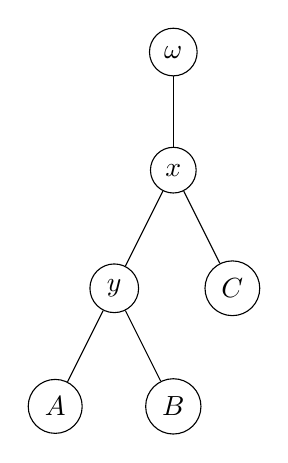
\begin{tikzpicture}[every node/.style={circle,draw},level distance=1.5cm, sibling distance=1.5cm]
    \node (w) {$\omega$}
        child {node (x) {$x$}
            child {node (y) {$y$}
                child {node (A) {$A$}}
                child {node (B) {$B$}}
            }
            child {node (C) {$C$}}
        };
    \end{tikzpicture}
    \quad
    \longrightarrow
    \quad
    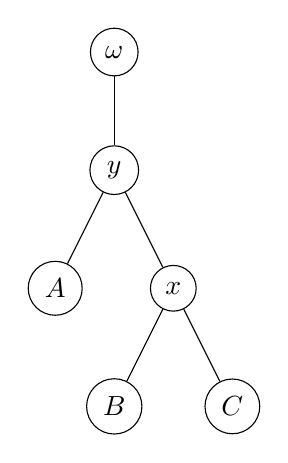
\begin{tikzpicture}[every node/.style={circle,draw},level distance=1.5cm, sibling distance=1.5cm]
    \node (w) {$\omega$}
        child {node (y) {$y$}
            child {node (A) {$A$}}
            child {node (x) {$x$}
                child {node (B) {$B$}}
                child {node (C) {$C$}}
            }
        };
    \end{tikzpicture}
    \]
\end{definition}

\subsection{Insert operation}

\newpage

\section{Hashing}
\subsection{Hash tables}
\begin{definition}
    A \textbf{hash table} uses a hash function to map keys from the universe of keys \( U \) to positions in an array of size \( m \) called buckets. 
    \begin{itemize}
        \item The key is stored in the appropriate bucket. 
        \item The number of keys stored is \( n \).
        \item The \textbf{load factor} \( \alpha \) is given by: $\alpha = \frac{n}{m}, \quad 0 < \alpha \leq 1$
        \begin{itemize}
            \item Expect $n \leq m$ so the places to store in the array is bigger than the number of keys to store in $n$.
        \end{itemize}
    \end{itemize}
\end{definition}

\subsection{Hash function}
\begin{definition}
    A \textbf{hash function} \( h(\text{key}) \) is used to convert a key into a numeric value, which is then used to index the array. 
    \begin{itemize}
        \item i.e. Maps a key in $U$ to an index from $0$ to $m-1$.
        \item A good hash function minimizes collisions, where two or more keys are assigned to the same index.
    \end{itemize}
\end{definition}

\subsection{Methods}
\subsubsection{Division Method}
\begin{definition}
    The \textbf{division method} computes the hash as:
    \[
    h(\text{key}) = \text{key} \mod m
    \]
    \begin{itemize}
        \item \( m \) is typically a prime number. 
    \end{itemize}
\end{definition}

\subsubsection{Multiplication Method}
\begin{definition}
The \textbf{multiplication method} computes the hash as:
\[
h(\text{key}) = \left\lfloor m \cdot ((\text{key} \cdot A) \mod 1) \right\rfloor
\]
\begin{itemize}
    \item \( A = \frac{\sqrt{5} - 1}{2} \), the golden ratio, is used to spread keys more evenly. 
    \item $m = 2^p$ are good values.  
\end{itemize}
\end{definition}

\subsection{Resolutions}
\subsubsection{Resolution by Chaining}
\begin{definition}
Resolves collisions by maintaining a linked list at each bucket. If two or more keys hash to the same index, they are stored in the same linked list.
\end{definition}

\subsubsection{Resolution by open addressing}
\begin{definition}
    Resolves collisions by probing for the next available slot in the table. 
    \begin{itemize}
        \item Instead of maintaining a list of keys at each bucket, each key is placed directly in the table, and a probing sequence is followed if collisions occur.
    \end{itemize}
    \end{definition}
    
    \subsubsection{Probing Methods}
    \begin{definition}
        \begin{enumerate}
            \item \textbf{Linear Probing:} Probe and insert next element:
            
            \[
            L_0 = h(\text{key})
            \]
            
            If the bucket is full (i.e., a collision), then we check the next slot in the table until an empty one is found (i.e., reprobe):
            
            \[
            L_{j+1} = (L_j + 1) \mod m
            \]
            
            \begin{itemize}
                \item However, linear probing can lead to \textbf{clustering}, where groups of keys form large contiguous blocks in the array.
            \end{itemize}
        
            \item \textbf{Double Hashing:} Using two hash functions to avoid clustering. If a collision occurs at index \(i_0\):
            
            \[
            L_1 = h_1(\text{key})
            \]
            
            The next probe location is computed by:
            
            \[
            L_{j+1} = (L_j + h_2(\text{key})) \mod m
            \]
            
            \begin{itemize}
                \item This results in better distribution of keys across the table and reduces clustering.
            \end{itemize}
        \end{enumerate}
    \end{definition}

\newpage

\section{Dynamic programming}
\begin{process}
    \begin{enumerate}
        \item Visualize example. 
        \item \textbf{Optimal substructure:} Characterize the structure of an optimal solution)
        \item \textbf{Recursive formula:} Find a relationship among sub-problems (i.e. defines the values of an optimal solution recursively in terms of the optimal solution to sub-problems)
        \begin{enumerate}
            \item Base case(s)
            \item Recursive formula 
        \end{enumerate}
        \item Compute the value of an optimal solution (bottom-up solving sub-problems in order or top-down solving problem recursively)
        \item \textbf{Time complexity:} $O(n^{\text{\# subproblems per choice}}) O(\text{\# choices})$
    \end{enumerate}
\end{process}

\subsection{How to prove optimal substructure?}
\begin{process}
    
\end{process}

\begin{example}
    
\end{example}
\newpage

\section{Greedy Algorithms}
\begin{process}
    \begin{enumerate}
        \item 
    \end{enumerate}
\end{process}

\begin{example}
    
\end{example}

\end{document}
